\chapter{ Pruebas}

\section{ Decimation}
En este capitulo solo se realizarán pruebas del método decimation puesto que ya realiza internamente uso de los demás métodos y genera el objetivo final del proyecto. Por tanto se analizarán los resultados de las pruebas obtenidas de la ejecución del método sobre tres mallas ply:
\begin{itemize}
	\item \textbf{sphere:} Contiene 840 caras y 422 vértices y se ve como en la figura \ref{fig:esfera_100.png}.
	\item \textbf{beethoven:} Contiene 5030 caras y 2521 vértices y se ve como en la figura \ref{fig:beethoven_100.png}.
	\item \textbf{big\_dodge:} Contiene 16646 caras y 8477 vértices y se ve como en la figura \ref{fig:coche_100.png}.
\end{itemize} 

\begin{figure} %con el [H] le obligamos a situar aquí la figura
	\centering
	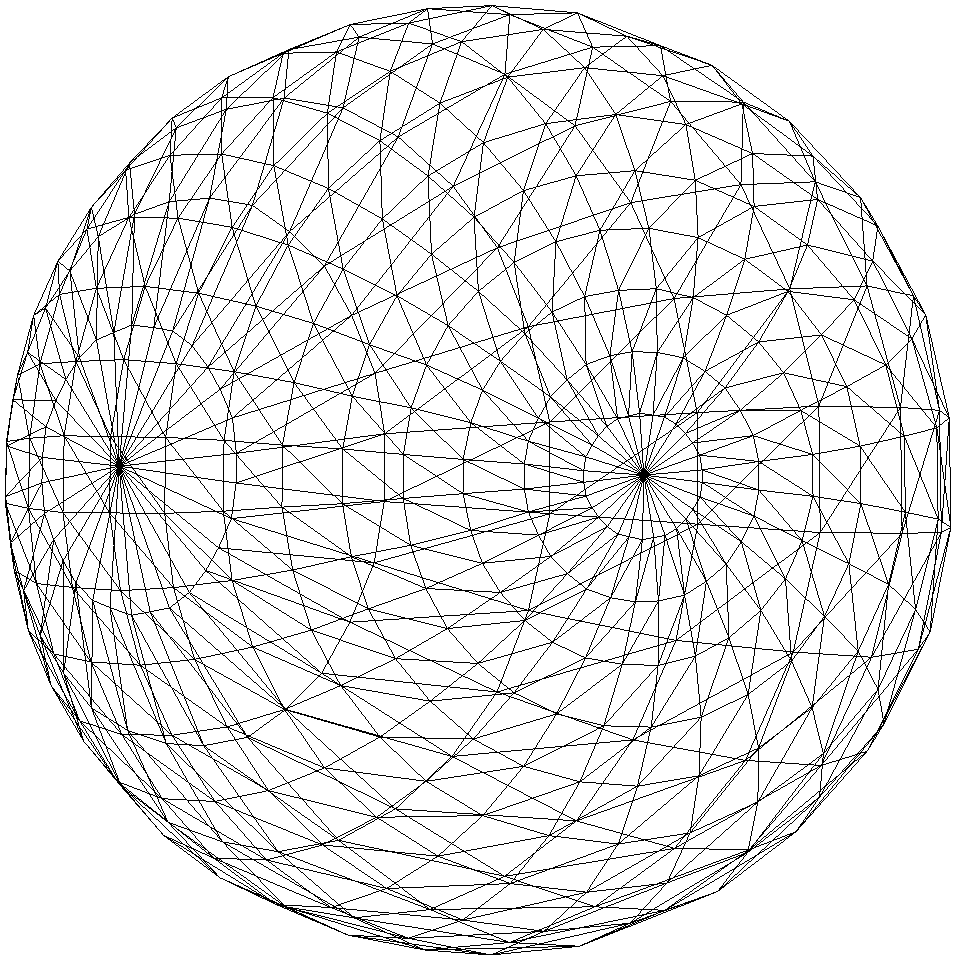
\includegraphics[scale=0.25]{imagenes/esfera_100.png} 
	\caption{Malla sphere.ply original.} \label{fig:esfera_100.png}
\end{figure}

\begin{figure} %con el [H] le obligamos a situar aquí la figura
	\centering
	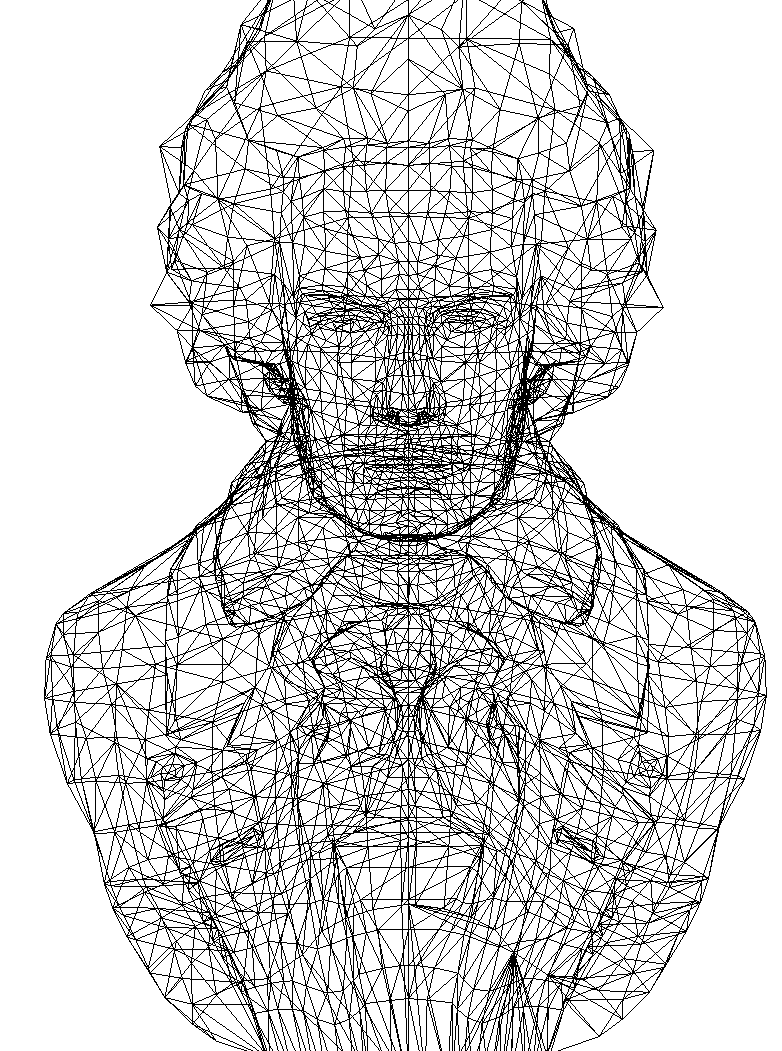
\includegraphics[scale=0.3]{imagenes/beethoven_100.png} 
	\caption{Malla beethoven.ply original.} \label{fig:beethoven_100.png}
\end{figure}

\begin{figure} %con el [H] le obligamos a situar aquí la figura
	\centering
	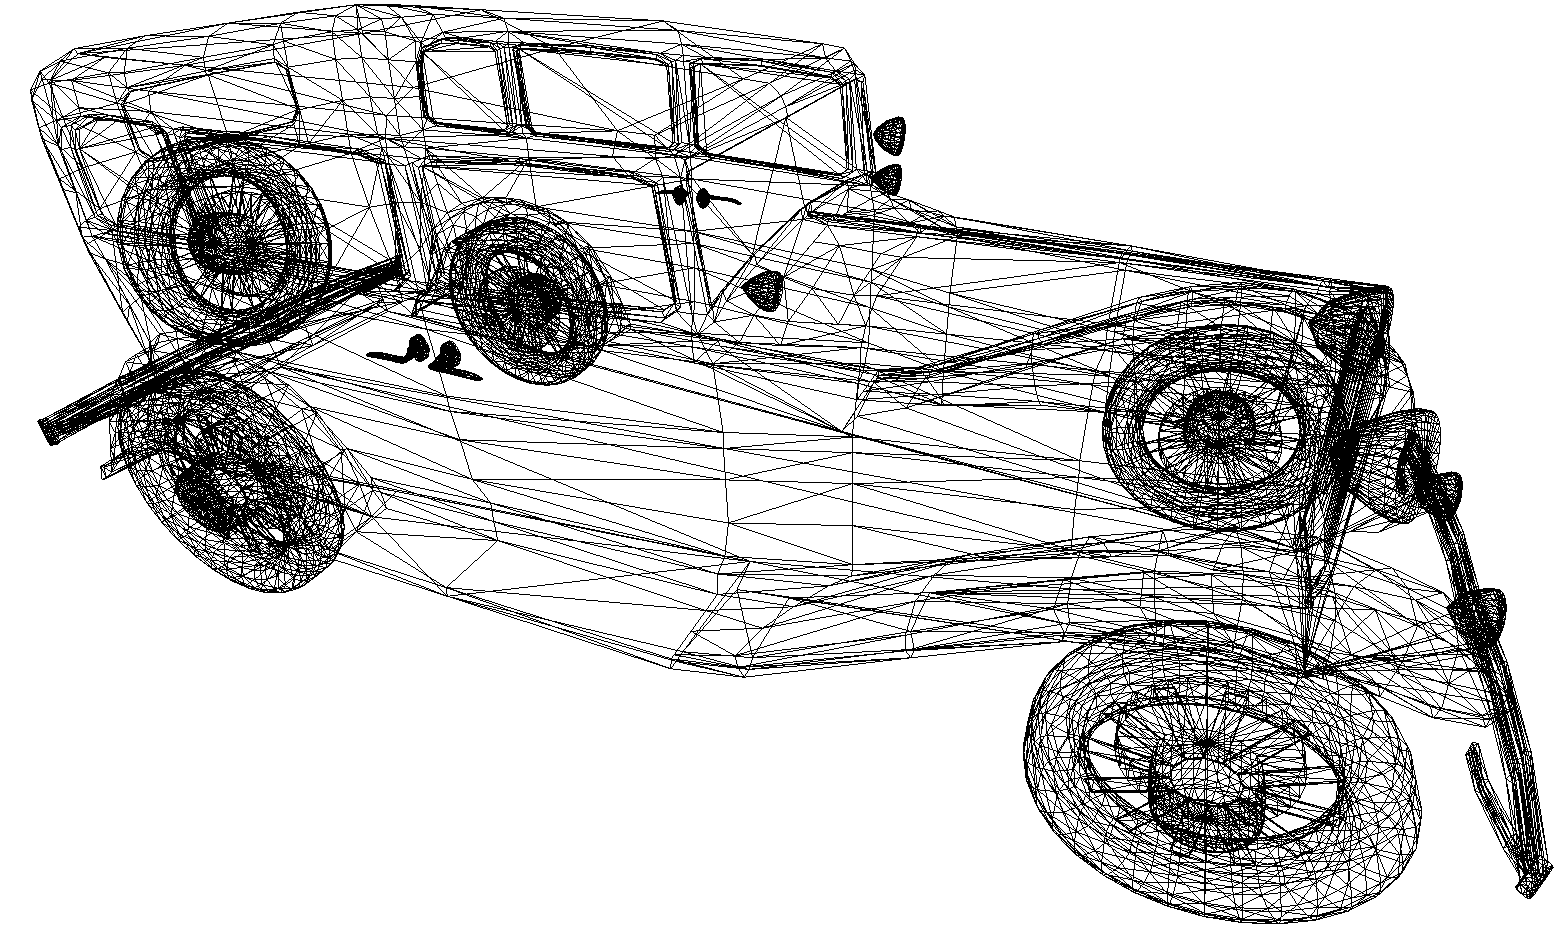
\includegraphics[scale=0.2]{imagenes/coche_100.png} 
	\caption{Malla big\_dodge.ply original.} \label{fig:coche_100.png}
\end{figure}

A estas mallas se les ha aplicado una tasa de reducción del 90\%, 75\%, 50\% y 25\%, y en cada tasa se ha obtenido el tiempo de computo del método \textit{decimation} y el número de caras obtenidas después de su aplicación. Todas las capturas de este capítulo se adjuntan a la memoria en la carpeta ``capturas'' con su resolución original. La tasa de reducción significa que la malla destino es ese porcentaje menos exacta a la original. Un ejemplo es una tasa de reducción al 90\% significa que la malla resultante tendrá un 10\% de error con respecto a la original y por tanto tendrá un 90\% menos de caras.

\newpage
\subsection{Sphere} 
Los resultados para la malla de Sphere que contiene una esfera han sido los siguientes.\\

Como se puede apreciar en la figura \ref{fig:esfera_90.png} donde solo se ha aplicado una tasa de reducción al 90\% la figura apenas se aprecia cambios significativos. Donde más se pueden apreciar la simplificación es en las tapas superior e inferior, aunque en la imagen de ven al frente y en la parte de atrás.\\ 

\begin{figure} %con el [H] le obligamos a situar aquí la figura
	\centering
	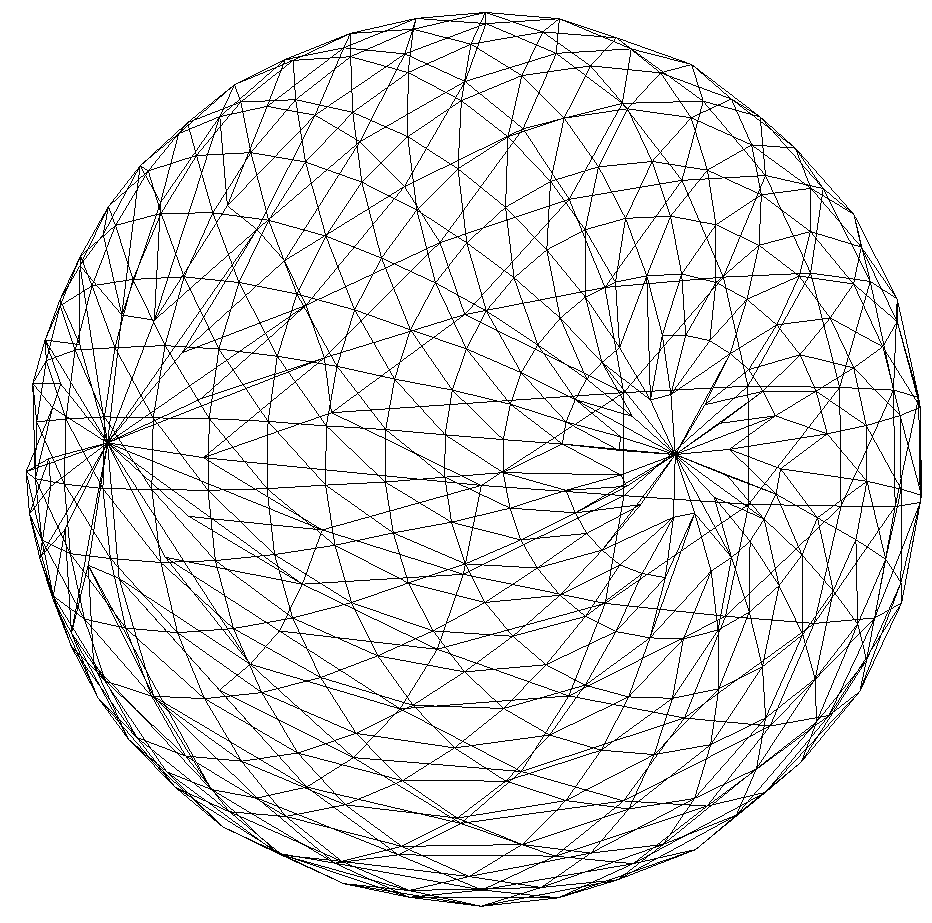
\includegraphics[scale=0.25]{imagenes/esfera_90.png} 
	\caption{Malla sphere.ply con una tasa de reducción del 90\%.} \label{fig:esfera_90.png}
\end{figure}

Si aplicamos ahora una tasa de reducción al 75\%, figura \ref{fig:esfera_75.png}, ya se puede apreciar cómo se empieza a deformar la esfera para ser más irregular, pero sigue manteniendo la silueta. Otro factor que se puede apreciar es que las primeras caras que se simplifican son las que forman las tapaderas superior e inferior, es decir, donde hay más caras pero más pequeñas que forman una superficie más homogénea al resto, con lo que se comprueba que el método simplifica primero las caras con que menor error van a producir.\\

\begin{figure} %con el [H] le obligamos a situar aquí la figura
	\centering
	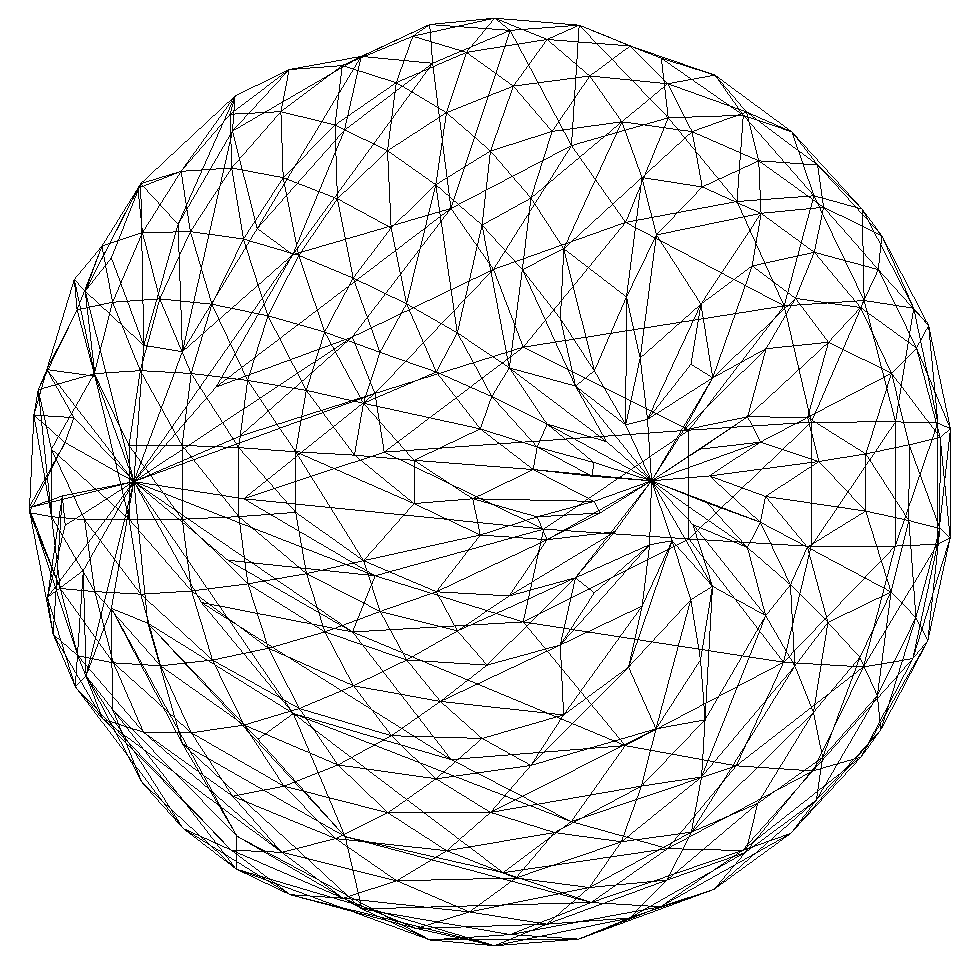
\includegraphics[scale=0.25]{imagenes/esfera_75.png} 
	\caption{Malla sphere.ply con una tasa de reducción del 75\%.} \label{fig:esfera_75.png}
\end{figure}

Aplicando una tasa de reducción más restrictiva al 50\%, figura \ref{fig:esfera_50.png}, ya la forma se compromete y aunque sigue manteniendo una silueta similar a una esfera. Las tapas superior e inferior ya han perdido su curvatura y pasan a ser lisas.\\

\begin{figure} %con el [H] le obligamos a situar aquí la figura
	\centering
	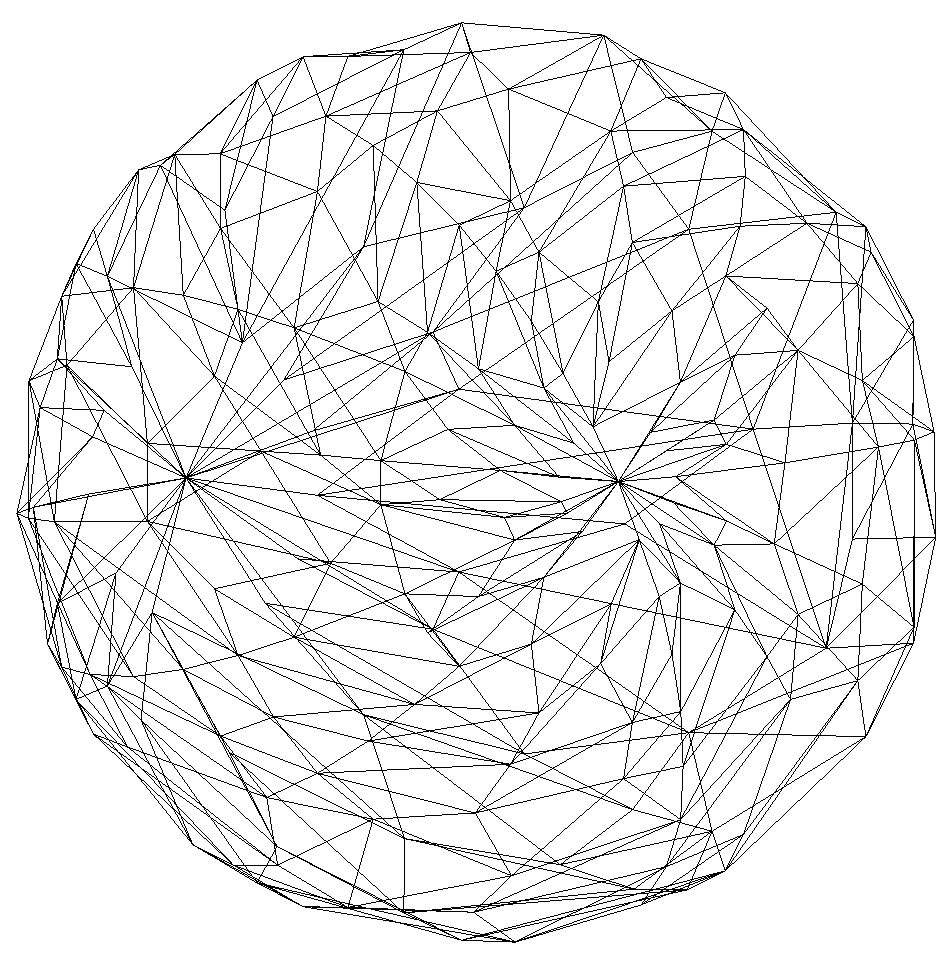
\includegraphics[scale=0.25]{imagenes/esfera_50.png} 
	\caption{Malla sphere.ply con una tasa de reducción del 50\%.} \label{fig:esfera_50.png}
\end{figure}

Con la tasa de reducción al 25\%, figura \ref{fig:esfera_25.png}, conseguimos una gran reducción en el número de caras, pero cuesta observar la similitud con una esfera perfectamente redonda.

\begin{figure} %con el [H] le obligamos a situar aquí la figura
	\centering
	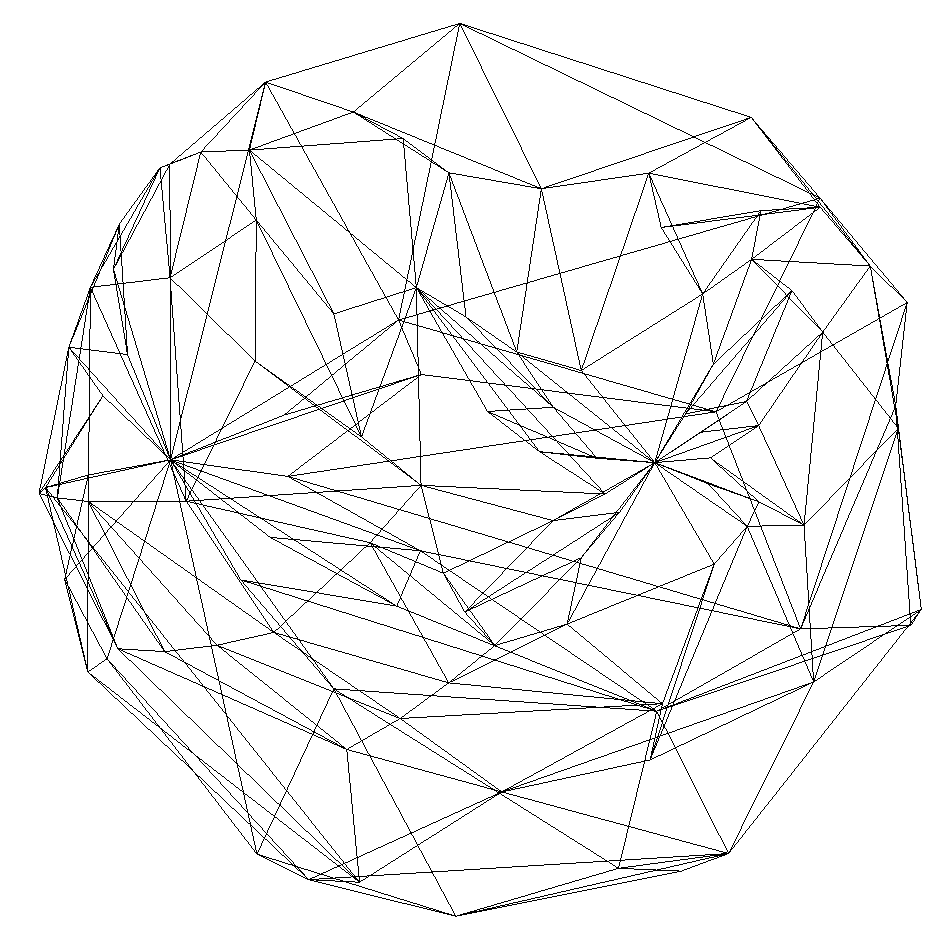
\includegraphics[scale=0.25]{imagenes/esfera_25.png} 
	\caption{Malla sphere.ply con una tasa de reducción del 25\%.} \label{fig:esfera_25.png}
\end{figure}

\subsection{Beethoven}
Cuando aplicamos las mismas tasas de reducción pero sobre una figura con un mayor número de elementos, obtenemos que la simplificación se realiza de manera más eficiente en cuanto a la similitud con la original. Puesto que al tener más zonas homogéneas esta figura la simplificación es más exacta.\\

\begin{figure} %con el [H] le obligamos a situar aquí la figura
	\centering
	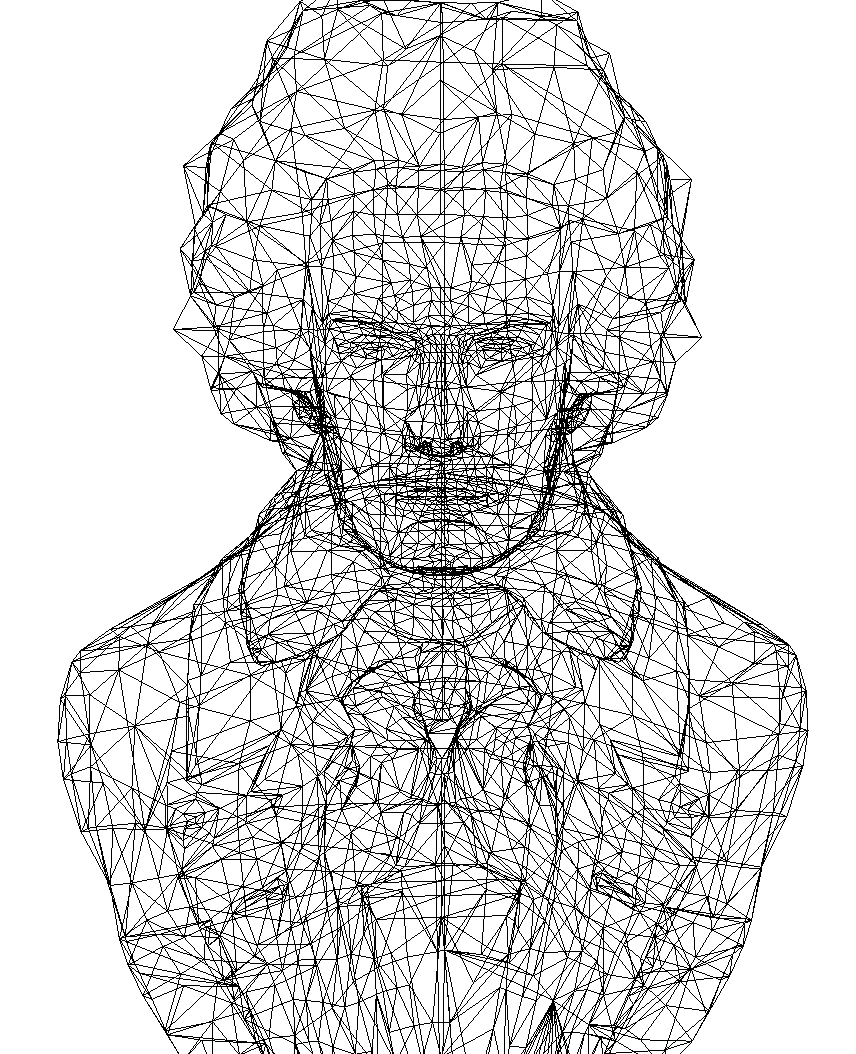
\includegraphics[scale=0.25]{imagenes/beethoven_90.png} 
	\caption{Malla beethoven.ply con una tasa de reducción del 90\%.} \label{fig:beethoven_90.png}
\end{figure}

En la primera simplificación, figura \ref{fig:beethoven_90.png} apenas notamos diferencia, al igual que en la esfera, una tasa de reducción alta consigue un resultado muy similar al original. Para ver los cambios tenemos que fijarnos en la parte baja de los hombros donde existe una zona de caras muy homogéneas y por tanto zonas más propensas a simplificarse.
\begin{figure} %con el [H] le obligamos a situar aquí la figura
	\centering
	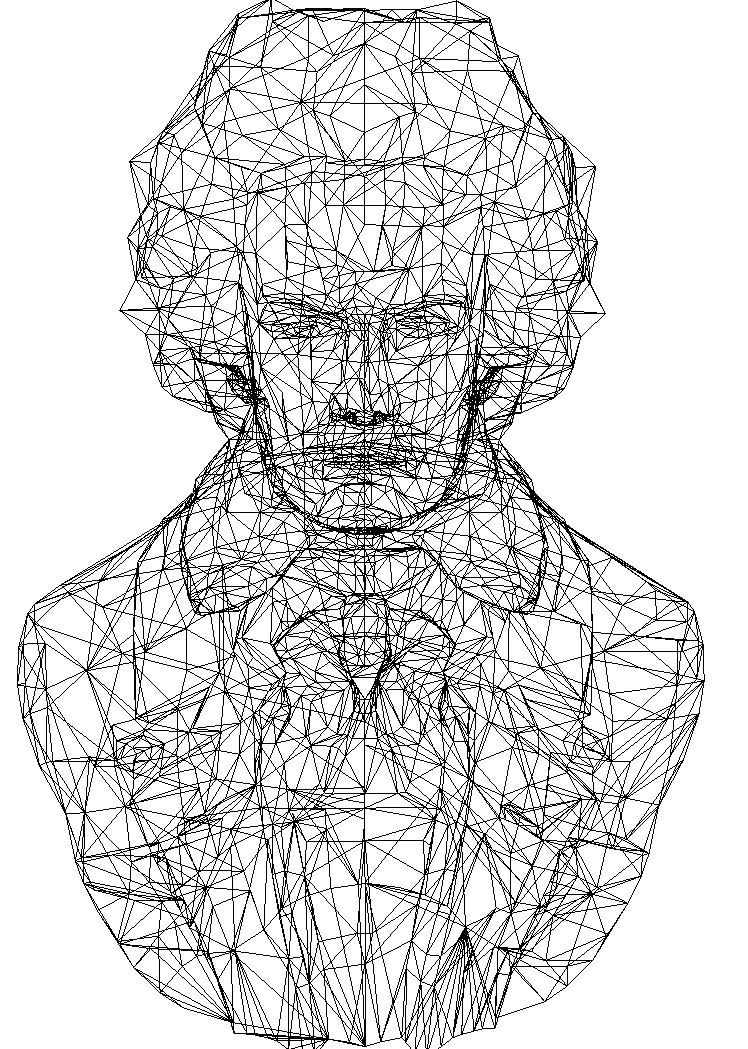
\includegraphics[scale=0.25]{imagenes/beethoven_75.png} 
	\caption{Malla beethoven.ply con una tasa de reducción del 75\%.} \label{fig:beethoven_75.png}
\end{figure}

Con la siguiente tasa de reducción al 75\%, figura \ref{fig:beethoven_75.png}, ya se empiezan a notar algunas partes menos definidas, pero solo apreciables si las comparamos con la original. Pero sigue manteniendo perfectamente la forma.\\
\begin{figure} %con el [H] le obligamos a situar aquí la figura
	\centering
	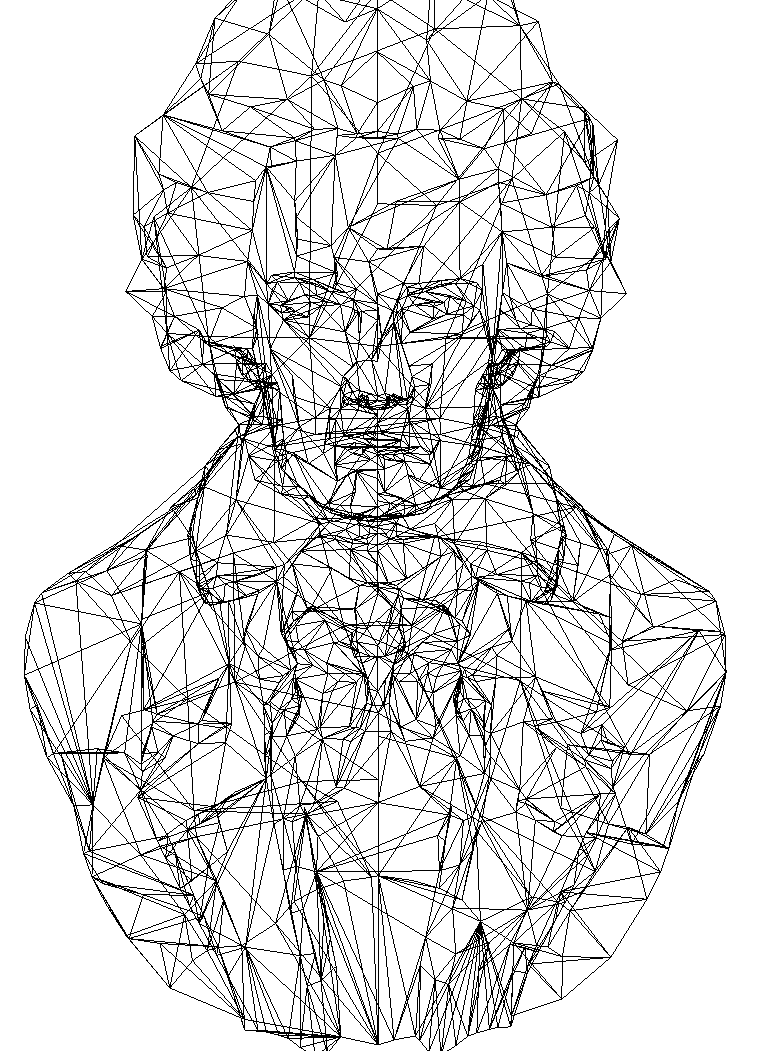
\includegraphics[scale=0.25]{imagenes/beethoven_50.png} 
	\caption{Malla beethoven.ply con una tasa de reducción del 50\%.} \label{fig:beethoven_50.png}
\end{figure}

Al aplicar la tasa de reducción al 50\%, figura \ref{fig:beethoven_50.png}, se produce un cambio significativo y ya se nota más la falta de calidad en la malla. Aunque sigue manteniendo la forma y se puede reconocer fácilmente la malla la cara ya no tiene la expresión original y muchos detalles se han perdido.\\

\begin{figure} %con el [H] le obligamos a situar aquí la figura
	\centering
	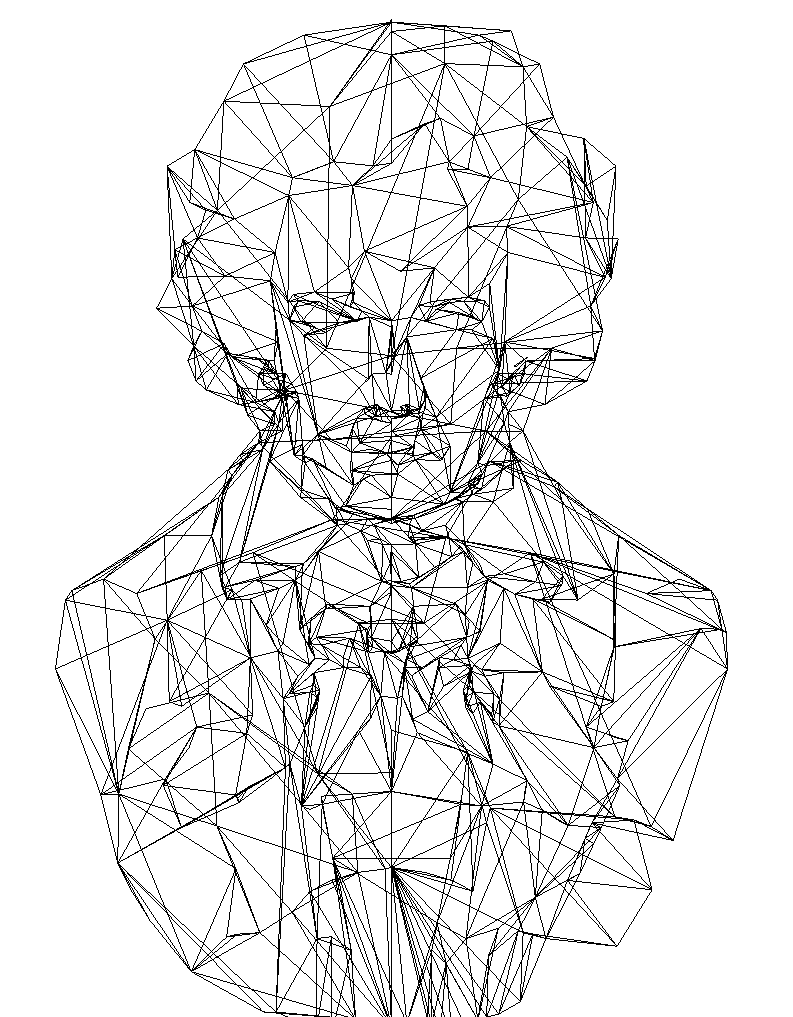
\includegraphics[scale=0.25]{imagenes/beethoven_25.png} 
	\caption{Malla beethoven.ply con una tasa de reducción del 25\%.} \label{fig:beethoven_25.png}
\end{figure}

Aplicando la última tasa de reducción al 25\%, figura \ref{fig:beethoven_25.png}, ya cuesta distinguir la figura y está muy poco definida.

\subsection{Big\_dodge}
Por último la malla con el mayor número de caras y con una característica más, que posee dos partes bien diferenciadas, una la carrocería del coche con superficies rectas y otra las ruedas y accesorios con una gran cantidad de ángulos y curvas. De está forma se podrá apreciar con más claridad la optimización del error conseguido en el método.\\

\begin{figure} %con el [H] le obligamos a situar aquí la figura
	\centering
	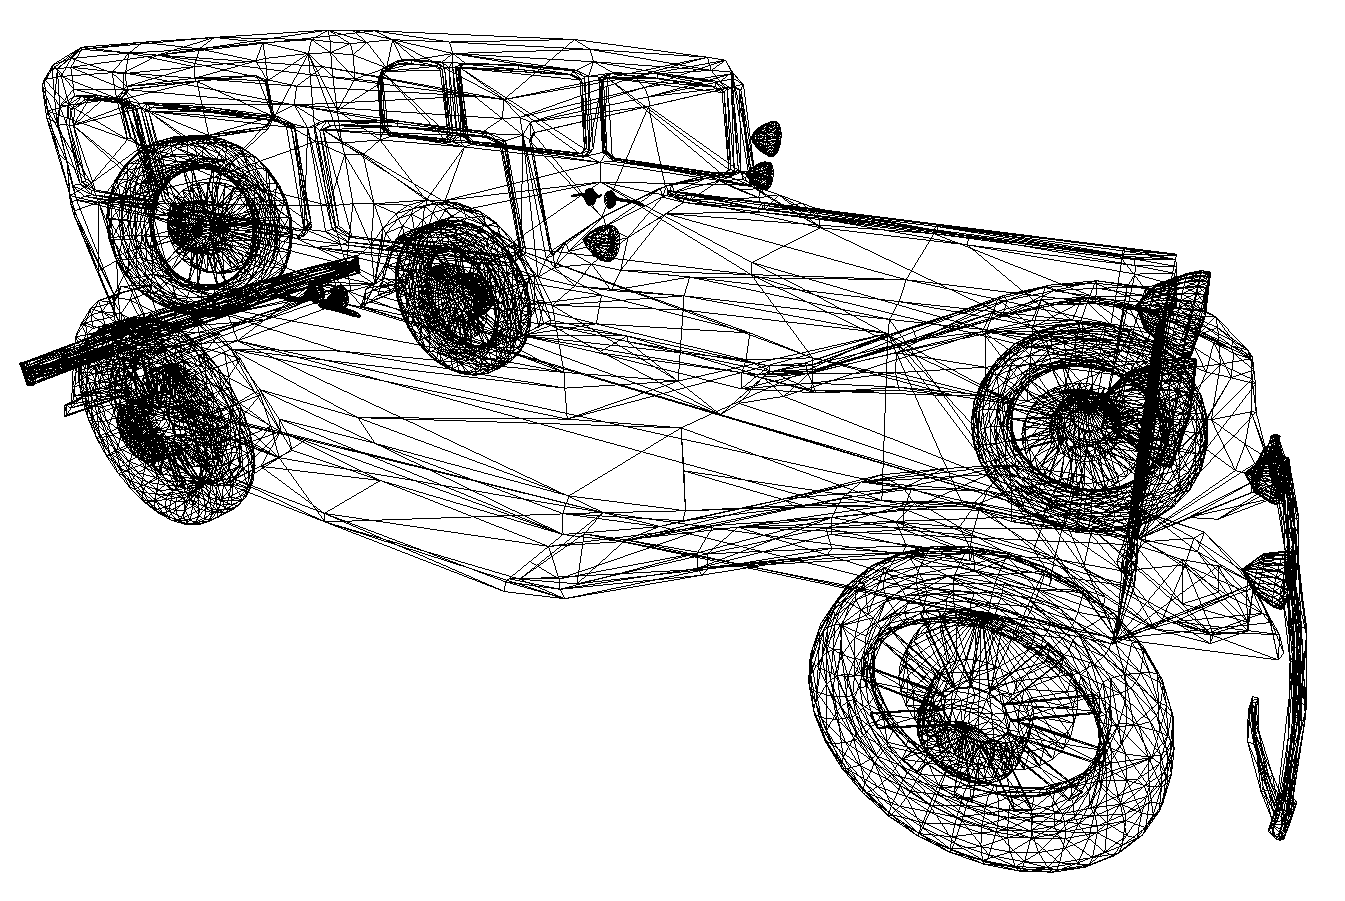
\includegraphics[scale=0.25]{imagenes/coche_90.png} 
	\caption{Malla big\_dodge.ply con una tasa de reducción del 90\%.} \label{fig:coche_90.png}
\end{figure}

En la primera simplificación, al 90\% figura \ref{fig:coche_90.png} los cambios son principalmente en la carrocería del coche donde los laterales ahora son caras más grandes y menos definidas. Se puede decir que el modelo no ha perdido a penas calidad.\\

\begin{figure} %con el [H] le obligamos a situar aquí la figura
	\centering
	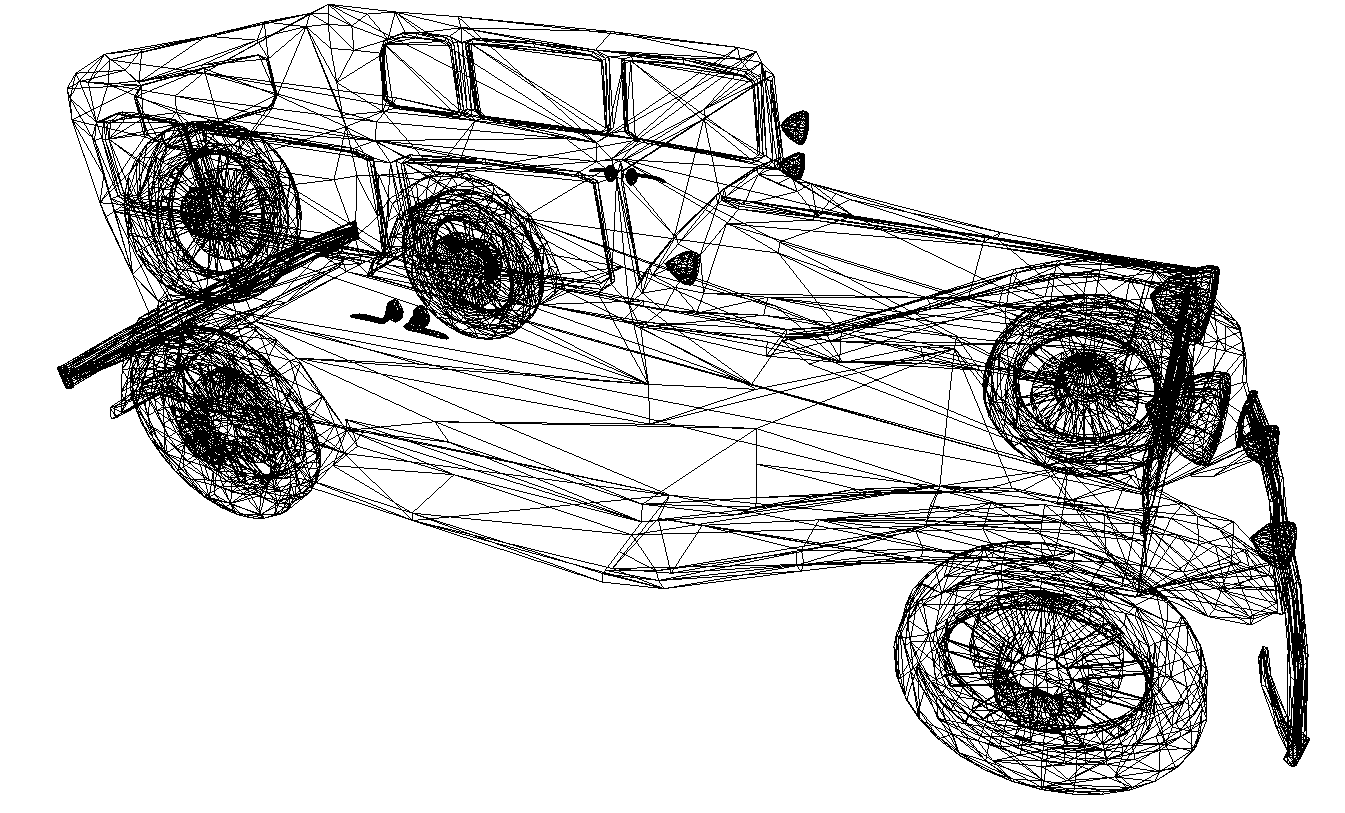
\includegraphics[scale=0.25]{imagenes/coche_75.png} 
	\caption{Malla big\_dodge.ply con una tasa de reducción del 75\%.} \label{fig:coche_75.png}
\end{figure}

En la segunda simplificación, al 75\% figura \ref{fig:coche_75.png}, los cambios en la carrocería son mayores y se empiezan a aplicar en las ruedas, en su lateral.\\

\begin{figure} %con el [H] le obligamos a situar aquí la figura
	\centering
	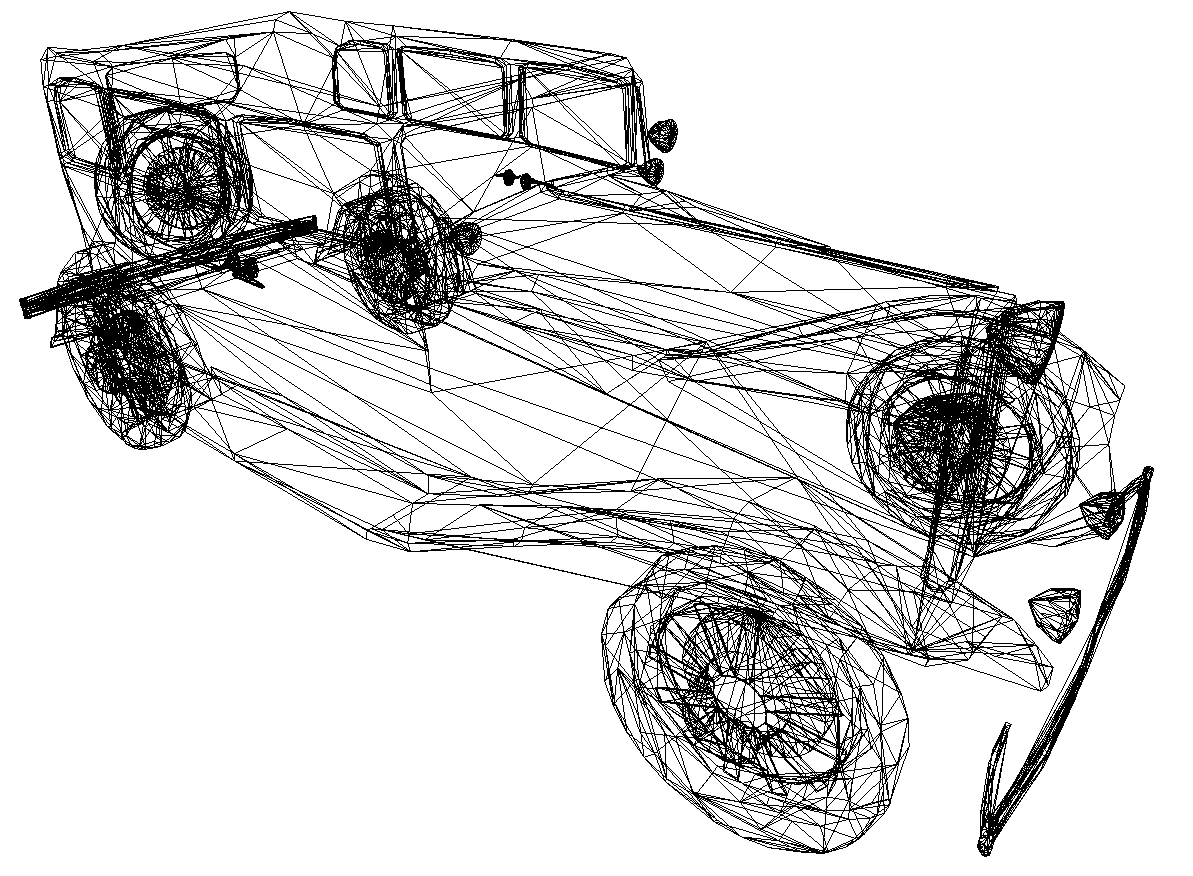
\includegraphics[scale=0.25]{imagenes/coche_50.png} 
	\caption{Malla big\_dodge.ply con una tasa de reducción del 50\%.} \label{fig:coche_50.png}
\end{figure}

Con la tercera simplificación, al 50\% figura \ref{fig:coche_50.png}, la forma se mantiene bastante bien y se ha concentrado la reducción en las ruedas y elementos algo más esféricos. Pero al igual que ocurría con Beethoven, el coche al tener muchos más elementos las simplificaciones permiten que se pueda simplificar más la malla sin perder mucha calidad.\\

\begin{figure} %con el [H] le obligamos a situar aquí la figura
	\centering
	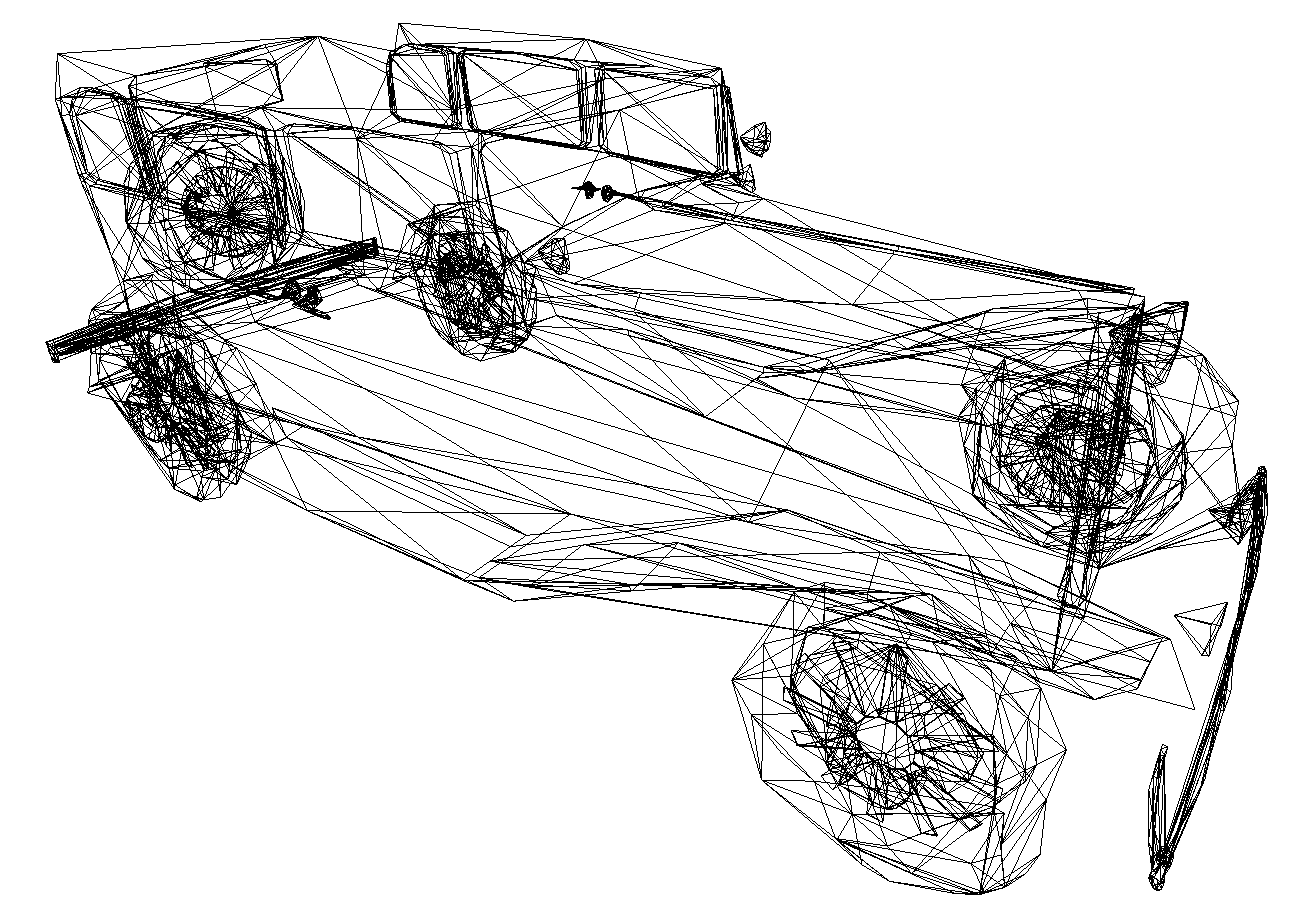
\includegraphics[scale=0.25]{imagenes/coche_25.png} 
	\caption{Malla big\_dodge.ply con una tasa de reducción del 25\%.} \label{fig:coche_25.png}
\end{figure}

En la cuarta y última simplificación, al 25\% figura \ref{fig:coche_25.png}, la estructura del coche ha quedado en grandes caras para cubrir la carrocería y los demás elementos se han simplificado en gran medida. Todavía se puede ver la forma de la malla original pero ya con mucha menos calidad.

\newpage
\subsection{Evaluación de las pruebas}
Como se comentó al principio del capítulo se han tomado los tiempos de ejecución del método \textit{decimation} al aplicarse cada una de las cuatro tasas de reducción y así poder comparar el costo en tiempo y el resultado obtenido, además para poder evaluar mejor el resultado se han obtenido el número de caras finales.\\

\begin{table}[]
	\centering
	\begin{tabular}{|l|l|l|l|}
		\hline
		\multicolumn{4}{|c|}{Tiempos de ejecución}     \\ \hline
		Reducción \% & big\_dodge & Bethoveen & sphere \\ \hline
		10           & 20,90      & 1,8       & 0,0423 \\ \hline
		25           & 46,80      & 3,68      & 0,0959 \\ \hline
		50           & 83,15      & 6,12      & 0,166  \\ \hline
		75           & 106,00     & 8,13      & 0,211  \\ \hline
	\end{tabular}
	\caption{Table de los tiempos de ejecución del método decimation sobre distintas mallas ply.}
	\label{tab:tiempos_decimation}
\end{table}

\begin{figure} %con el [H] le obligamos a situar aquí la figura
	\centering
	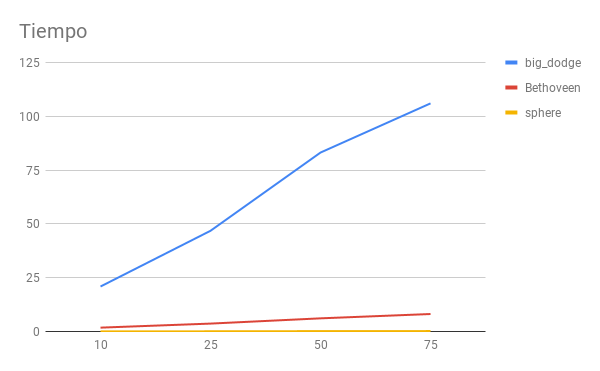
\includegraphics[scale=0.5]{imagenes/Tiempo.png} 
	\caption{Gráfica de la tabla \ref{tab:tiempos_decimation}, que muestra el aumento de costo al agrandar la tasas de } \label{fig:tiempo.png}
\end{figure}

En la tabla \ref{tab:tiempos_decimation} se puede observar como los tiempos de aplicación del método se incrementan en gran medida con forme aplicamos tasas de reducción más restrictivas. En la gráfica \ref{fig:tiempo.png} vemos como las mallas con menor número de elementos siguen un crecimiento moderado, mientras que la malla big\_dodge sigue un crecimiento prácticamente lineal. Esto es una relación directa entre el número de elementos a evaluar, pero recordemos que también se consigue una mayor calidad.\\

También hemos considerado el número de caras resultantes, que se puede observar en la tabla \ref{tab:caras} el número de caras es proporcional a la tasas de reducción. Esta relación se mantiene constante. Como el caso de las tasas al 90\% donde la calidad de la malla no se veía muy afectada y donde el número de caras es algo menor, esto es importante tenerlo en cuenta ya que para aplicar en un futuro la técnica de Level Of Details, todo lo que se pueda ahorrar en elementos sin comprometer mucho la calidad es una gran solución.

\begin{table}[]
	\centering
	\begin{tabular}{|r|c|c|c|}
		\hline
		\multicolumn{4}{|c|}{Número de Triángulos}                                                                                          \\ \hline
		\multicolumn{1}{|l|}{Reducción \%} & \multicolumn{1}{l|}{big\_dodge} & \multicolumn{1}{l|}{Bethoveen} & \multicolumn{1}{l|}{sphere} \\ \hline
		0                                  & 16.646                          & 5.030                          & 840                         \\ \hline
		10                                 & 14.982                          & 4.528                          & 756                         \\ \hline
		25                                 & 12.484                          & 3.772                          & 630                         \\ \hline
		50                                 & 8.324                           & 2.516                          & 420                         \\ \hline
		75                                 & 4.162                           & 1.258                          & 210                         \\ \hline
	\end{tabular}
	\caption{Tabla de número de caras sobre las mallas con distintos tipos de tasas de reducción}
	\label{tab:caras}
\end{table}

Por último es necesario analizar el tiempo entre figuras con respecto al número de caras de cada figura. En la tabla \ref{tab:inc_coche_beethoven}, tenemos en la segunda (Inc. Caras) columna el incremento de caras que existe entre la malla big\_dodge y Beethoven y en la tercera columna (Inc. Tiempo). La primera columna nos muestra que la proporción de caras es constante entre una malla y la otra, pero en la segunda columna nos indica que el factor tiempo crece cuanto mayor es la tasas de reducción. Si comparamos ambos resultados obtenemos la última columna (Diferencia) que indica la diferencia entre el aumento de caras y el aumento del tiempo, por tanto el factor tiempo crece mucho al aumentar el número de elementos a evaluar, crece por del orden de 9 veces por encima del aumento del número de caras.

\begin{table}[]
	\centering
\begin{tabular}{l|c|c|c|}
	\cline{2-4}
	Reducción \% & Inc. Caras  & \multicolumn{1}{l|}{Inc. Tiempo} & \multicolumn{1}{l|}{Diferencia} \\ \cline{2-4} 
	10           & 3,309343936 & 11,61111111                      & 8,301767175                     \\ \cline{2-4} 
	25           & 3,308745583 & 12,7173913                       & 9,408645721                     \\ \cline{2-4} 
	50           & 3,309650053 & 13,58660131                      & 10,27695125                     \\ \cline{2-4} 
	75           & 3,308426073 & 13,03813038                      & 9,729704308                     \\ \cline{2-4} 
\end{tabular}
	\caption{Tabla de diferencia entre el incremento de tiempo y el incremento de caras entre la malla de Big\_dodge y Beethoven.}
	\label{tab:inc_coche_beethoven}
\end{table}